\documentclass[tikz,border=2pt]{standalone}

\usepackage{pgfplots}
\usepgfplotslibrary{groupplots}
\usetikzlibrary{arrows.meta}
\pgfplotsset{compat=1.18}
\definecolor{cbBlue}{HTML}{0072B2}
\definecolor{cbOrange}{HTML}{D55E00}
\definecolor{cbGreen}{HTML}{009E73}
\definecolor{cbPurple}{HTML}{CC79A7}
\definecolor{cbSky}{HTML}{56B4E9}
\definecolor{cbGold}{HTML}{E69F00}
\pgfplotsset{
  paperaxis/.style={
    axis line style={black!65,line width=0.45pt},
    tick style={black!65,line width=0.45pt},
    tick label style={font=\footnotesize},
    label style={font=\small},
    title style={font=\small\bfseries,yshift=-1pt},
    grid=major,
    grid style={black!10,line width=0.35pt},
    line width=1.05pt,
    mark size=1.8pt,
  }
}

\begin{document}
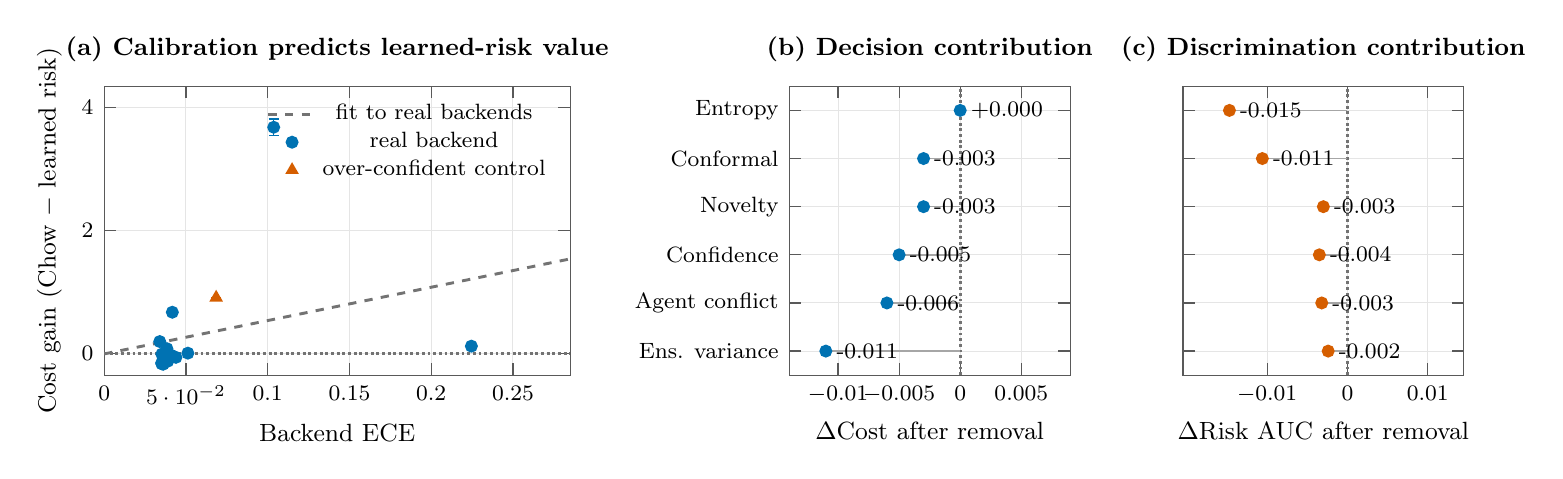
\begin{tikzpicture}
\begin{axis}[
  paperaxis,
  name=eceplot,
  width=7.5cm,height=5.25cm,
  xmin=0,xmax=0.285,ymin=-0.35,ymax=4.35,
  xlabel={Backend ECE},
  ylabel={Cost gain (Chow $-$ learned risk)},
  title={(a) Calibration predicts learned-risk value},
  legend style={font=\footnotesize,draw=none,fill=none,at={(0.98,0.98)},anchor=north east,row sep=-1pt},
]
\addplot[black!55,dashed,domain=0:0.285,samples=2] {5.4253*x - 0.0044};
\addlegendentry{fit to real backends}
\addplot[only marks,mark=*,cbBlue,fill=cbBlue,error bars/.cd,y dir=both,y explicit]
table[row sep=\\,x=ece,y=gain,y error=err]{
ece gain err\\
0.0361 -0.172 0.006\\
0.0353 -0.008 0.001\\
0.0512 0.008 0.0\\
0.0384 0.081 0.0\\
0.0417 0.674 0.0\\
0.0353 -0.165 0.0\\
0.0439 -0.06 0.003\\
0.034 0.197 0.0\\
0.1037 3.684 0.135\\
0.0409 -0.025 0.034\\
0.2246 0.122 0.0\\
0.0389 -0.123 0.005\\
0.0352 -0.151 0.0\\
};
\addlegendentry{real backend}
\addplot[only marks,mark=triangle*,cbOrange,fill=cbOrange,error bars/.cd,y dir=both,y explicit]
table[row sep=\\,x=ece,y=gain,y error=err]{
ece gain err\\
0.0685 0.912 0.0\\
};
\addlegendentry{over-confident control}
\addplot[black!55,densely dotted,domain=0:0.285,samples=2] {0};
\end{axis}

\begin{axis}[
  paperaxis,
  % Reserve a real label gutter: the longest row name (Agent conflict) must
  % not intrude into panel (a), especially after the figure is scaled in IEEE.
  at={(8.70cm,0)},anchor=south west,
  width=5.15cm,height=5.25cm,
  xmin=-0.014,xmax=0.009,ymin=0.5,ymax=6.5,
  xlabel={$\Delta$Cost after removal},
  title={(b) Decision contribution},
  ytick={1,2,3,4,5,6},
  yticklabels={Ens. variance,Agent conflict,Confidence,Novelty,Conformal,Entropy},
  xtick={-0.01,-0.005,0,0.005},
  scaled x ticks=false,
  /pgf/number format/fixed,
  /pgf/number format/precision=3,
]
\addplot[black!55,densely dotted] coordinates {(0,0.5) (0,6.5)};
\addplot[black!35,line width=.55pt] coordinates {(0,6) (0.0000,6)};
\addplot[black!35,line width=.55pt] coordinates {(0,5) (-0.0030,5)};
\addplot[black!35,line width=.55pt] coordinates {(0,4) (-0.0030,4)};
\addplot[black!35,line width=.55pt] coordinates {(0,3) (-0.0050,3)};
\addplot[black!35,line width=.55pt] coordinates {(0,2) (-0.0060,2)};
\addplot[black!35,line width=.55pt] coordinates {(0,1) (-0.0110,1)};
\addplot[only marks,mark=*,cbBlue,fill=cbBlue] coordinates {(0.0000,6) (-0.0030,5) (-0.0030,4) (-0.0050,3) (-0.0060,2) (-0.0110,1)};
\node[font=\footnotesize,anchor=west] at (axis cs:0.0000,6) {+0.000};
\node[font=\footnotesize,anchor=west] at (axis cs:-0.0030,5) {-0.003};
\node[font=\footnotesize,anchor=west] at (axis cs:-0.0030,4) {-0.003};
\node[font=\footnotesize,anchor=west] at (axis cs:-0.0050,3) {-0.005};
\node[font=\footnotesize,anchor=west] at (axis cs:-0.0060,2) {-0.006};
\node[font=\footnotesize,anchor=west] at (axis cs:-0.0110,1) {-0.011};
\end{axis}

\begin{axis}[
  paperaxis,
  at={(13.70cm,0)},anchor=south west,
  width=5.15cm,height=5.25cm,
  xmin=-0.0205,xmax=0.0145,ymin=0.5,ymax=6.5,
  xlabel={$\Delta$Risk AUC after removal},
  title={(c) Discrimination contribution},
  ytick={1,2,3,4,5,6},yticklabels={,,,,,},
  xtick={-0.01,0,0.01},
  scaled x ticks=false,
  /pgf/number format/fixed,
  /pgf/number format/precision=3,
]
\addplot[black!55,densely dotted] coordinates {(0,0.5) (0,6.5)};
\addplot[black!35,line width=.55pt] coordinates {(0,6) (-0.0147,6)};
\addplot[black!35,line width=.55pt] coordinates {(0,5) (-0.0106,5)};
\addplot[black!35,line width=.55pt] coordinates {(0,4) (-0.0030,4)};
\addplot[black!35,line width=.55pt] coordinates {(0,3) (-0.0035,3)};
\addplot[black!35,line width=.55pt] coordinates {(0,2) (-0.0032,2)};
\addplot[black!35,line width=.55pt] coordinates {(0,1) (-0.0024,1)};
\addplot[only marks,mark=*,cbBlue,fill=cbBlue] coordinates {};
\addplot[only marks,mark=*,cbOrange,fill=cbOrange] coordinates {(-0.0147,6) (-0.0106,5) (-0.0030,4) (-0.0035,3) (-0.0032,2) (-0.0024,1)};
\node[font=\footnotesize,anchor=west] at (axis cs:-0.0147,6) {-0.015};
\node[font=\footnotesize,anchor=west] at (axis cs:-0.0106,5) {-0.011};
\node[font=\footnotesize,anchor=west] at (axis cs:-0.0030,4) {-0.003};
\node[font=\footnotesize,anchor=west] at (axis cs:-0.0035,3) {-0.004};
\node[font=\footnotesize,anchor=west] at (axis cs:-0.0032,2) {-0.003};
\node[font=\footnotesize,anchor=west] at (axis cs:-0.0024,1) {-0.002};
\end{axis}
\end{tikzpicture}
\end{document}
